The previous two chapters described a recoverable persistent queue data structure as well as three memory persistency models.
This chapter uses the queue and models to motivate the need for relaxed memory persistency models.
First, I describe the methodology used for this evaluation.

\section{Methodology}
\label{sec:PersistencyEval:Methodology}

To evaluate persistent queue designs and persistency models I measure instruction execution rate on a real server and persist concurrency via memory traces.
All experiments run the queue benchmarks optimized for volatile performance.
Memory padding is inserted to objects and queue inserts to provide 64-byte alignment to prevent false sharing.
%All threads are constrained to a single socket using the Linux \emph{taskset} utility.
Critical sections are implemented using MCS locks \cite{Mellor-Crummey91}, a high-throughput queue based lock.
Experiments insert 100-byte queue entries.
%Once the queue fills a thread flash-clears the queue by copying the entire valid portion of the data segment at once and updating the circular buffer tail pointer, simulating an archive process.
%Archiving in this manner minimizes interference between archive threads and inserting threads that would otherwise increase lock contention increase persist ordering constrain critical path.
Instruction execution rate is measured as inserts per second while inserting 100,000,000 entries between all threads using an Intel Xeon E5645 processor (2.4GHz).
The remainder of this section describes how I measure persist concurrency for the queue benchmarks.

\textbf{Persist Ordering Constraint Critical Path.}
Instead of proposing specific hardware designs and using architectural simulation, I instead measure, via memory traces, the persist ordering constraint critical path.
The evaluation assumes a memory system with infinite bandwidth and memory banks (so bank conflicts never occur), but with finite persist latency.
Thus, persist throughput is limited by the longest chain (critical path) of persist ordering constraints observed by execution under different memory persistency models.
While real memory systems must necessarily delay elsewhere due to limited bandwidth, bank conflicts, and other memory-related delays incurred in the processor, measuring persist ordering constraint critical path offers an implementation-independent measure of persist concurrency.

%Measuring persist critical path still requires several assumptions about the memory system.
I measure persist critical path under the following assumptions.
Every persist to the persistent address space occurs in place (there is no hardware support for logging or indirection to allow concurrent persists).
I track persist dependences at variable granularity (e.g., eight-byte words or 64-byte cache lines).
Coarse-grained persist tracking is susceptible to false sharing, introducing unnecessary persist ordering constraints due to accesses to the same cache line but not to overlapping addresses.
I similarly track persist coalescing with variable granularity.
Every persist attempts to coalesce with the last persist to that address.
A persist successfully coalesces if the persist fits within an atomically persistable memory block and coalescing with the previous persist to the same block does not violate any persist order constraints.
%Both persist dependence tracking and coalescing occurs within aligned blocks of memory.
%Using these assumptions, we generate memory access traces and simulate persist timing to determine persist ordering constraint critical path.

\textbf{Memory Trace Generation.}
I use PIN to instrument the queue benchmarks and generate memory access traces \cite{LukCohn05}.
Tracing multi-threaded applications requires additional work to ensure analysis-atomicity---application instructions and corresponding instrumentation instructions must occur atomically, otherwise the traced memory order will not accurately reflect execution's memory order.
I provide analysis atomicity by creating a bank of locks and assigning every memory address (or block of addresses) to a lock.
Each instruction holds all locks corresponding to its memory operands while being traced.
%Locks are numbered and acquired in lock number-order to avoid deadlocks.
%In addition to tracing memory accesses, we instrument the queue benchmarks with region-of-interest markers, persist barriers, and persistent malloc/free to distinguish persistent and volatile address spaces.
%Each annotation is implemented as a standard function and instrumented in PIN.
In addition to tracing memory accesses, I instrument the queue benchmarks with persist barriers and persistent malloc/free to distinguish volatile and persistent address spaces.
My tracing infrastructure is publicly available \cite{AtomicMemoryTrace}.

Tracing memory accesses in such a way ensures that the trace accurately reflects the order of memory accesses from execution.
%However, as only one instruction from any thread can access each memory region at once, and instructions on each thread occur in program order, our trace is limited to SC.
As only one instruction from any thread can access each address at once, and instructions on each thread occur in program order, the trace observes SC.
Thus, all evaluated memory persistency models assume SC as the underlying consistency model.

\textbf{Performance Validation.}
It is important that tracing not heavily influence thread interleaving, which would affect persist concurrency.
I measure the distance of insert operations between successive inserts from the same thread.
I observe that the distribution of insert distance is the same when running each queue natively and with instrumentation enabled, suggesting that thread interleaving is not significantly affected.

\textbf{Persist Timing Simulation.}
%Using the memory trace we measure persist ordering constraint critical path as the time of the last persist from any thread.
Persist times are tracked per address (both persistent and volatile) as well as per thread according to the persistency model.
For example, under strict persistency each persist occurs after or coalesces with the most recent persists observed through (1) each load operand, (2) the last store to the address being overwritten, and (3) any persists observed by previous instructions on the same thread.
Persists' ability to coalesce is similarly propagated through memory and thread state to determine when coalescing will violate persist ordering constraints---a persist may coalesce if its most recent persist dependence (greatest timestamp) occurs to the same atomically persistable memory block and all other persist dependences are strictly older (timestamp strictly less).
Under such situations coalescing will not violate any of the earlier persist dependences.
The persistency models differ as to the events that propagate persist ordering constraints through memory and threads.

Next, I use this methodology to establish the need for relaxed persistency models, as well as measure their opportunity to accelerate recoverable systems.

\section{Evaluation}
\label{sec:PersistencyEval:Evaluation}

This section uses the previously described methodology to demonstrate that persist ordering constraints present a performance bottleneck under strict persistency.
However, relaxed persistency improves persist concurrency, removing stalls caused by persists.
I also show that relaxed persistency models are resilient to large persist latency, allowing maximum throughput as persist latency increases.
Finally, I consider the effects of larger atomic persists and coarse-grained persist dependence tracking. 

\subsection{Relaxed Persistency Performance}
\label{section:Evaluation:PersistencyPerformance}

NVRAM persists are only a concern if they slow down execution relative to non-recoverable systems.
If few enough persists occur, or those persists are sufficiently concurrent, performance remains bounded by the rate that instructions execute with few delays caused by persists.
To determine system performance, I assume that only one of the instruction execution rate and persist rate is the bottleneck: either the system executes at its instruction execution rate (measured on current hardware), or throughput is limited solely by persist rate (while observing persist dependencies and retaining recovery correctness).

\begin{table*}
  \centering
  \begin{tabular}{ l l l l l l l l l l }
    \hline
    Threads & \multicolumn{3}{c}{Copy While Locked} & \multicolumn{3}{c}{Two-Lock Concurrent} & \multicolumn{3}{c}{Queue Holes} \\
    & Strict & Epochs & Strands & Strict & Epochs & Strands & Strict & Epochs & Strands \\
    \hline \hline
    %1 & 0.03402668948225257 & 0.17329066524439704 & 12.395878787878786 & 0.07956161591630416 & 0.5569551810923878 & 28.931290043290044 & 0.03243921666510665 & 0.17329066524439704 & 13.36387317909169 \\
    %8 & 0.05787677206992028 & 3.167189491481337 & 21.084432900432898 & 0.4319337035691424 & 3.3529680365296803 & 21.615757575757577 & 0.2539605628870943 & 1.9442439473904665 & 19.535723905723902 \\
    1 & 0.034 & 0.17 & \textbf{12} & 0.080 & 0.56 & \textbf{29} & 0.032 & 0.17 & \textbf{13} \\
    8 & 0.058 & \textbf{3.2} & \textbf{21} & 0.43 & \textbf{3.4} & \textbf{22} & 0.25 & \textbf{1.9} & \textbf{20} \\
    \hline
  \end{tabular}
  \caption{
    \textbf{Relaxed Persistency Performance.}
    Persist-bound insert rate normalized to instruction execution rate assuming 500ns persist latency.
    System throughput is limited by the lower of persist and instruction rates---at greater than 1 (bold) instruction rate limits throughput; at lower than 1 execution is limited by the rate of persists.
    While strict persistency limits throughput, persist epochs maximizes performance for many threads and persist strands are necessary to maximize performance with one thread.
  }
  \label{table::RelaxedPerformance}
\end{table*}


Table~\ref{table::RelaxedPerformance} shows the achievable throughput for the queue benchmarks and persistency models for both one and eight threads assuming 500ns persists.
Rates are normalized to instruction execution---normalized rates above one (bold) admit sufficient persist concurrency to achieve the instruction execution rate while normalized rates below one are limited by persists.
Instruction execution rates vary between log version and number of threads (not shown).

Strict persistency, the most conservative model, falls well below instruction execution rate, suggesting that memory systems with such restrictive models will be persist-bound.
\emph{Copy While Locked} with one thread suffers nearly a 30$\times$ slowdown; over-constraining persist order greatly limits workload throughput.
%The leftmost bar represents strict persistency with SC, our most conservative model.
%The achievable throughput for this model sits well below the instruction execution rate, suggesting that a memory system using such restrictive models will be persist-bound.
%\emph{Copy While Locked} with one thread sees a 30$\times$ slowdown relative to instruction execution rate; over-constraining persist order greatly limits workload throughput.

Relaxing persistency improves throughput for persist-bound configurations.
Epoch persistency improves persist concurrency by allowing entire queue entries to persist concurrently and removes a number of unnecessary persist constraints via intentional persist epoch races.
All queue designs see a substantial increase in throughput, with the eight thread configurations achieving instruction execution rate.
At the same time, the one thread configurations remain persist-bound and their throughput suffers relative to a nonrecoverable system.
Nevertheless, \emph{Copy While Locked} with one thread is now only $5.9\times$ slower than the instruction execution rate.

While execution for all queue designs with many threads is already compute bound and does not benefit from further relaxing persistency, the single thread configurations require additional persist concurrency to improve performance.
Strand persistency allows concurrent persists from the same thread while still ensuring correct recovery.
This model enables incredibly high persist concurrency such that all log versions are compute-bound even for a single thread.
Sufficiently relaxed persistency models allow data structures and systems that recover from failure while retaining the throughput of existing main-memory data structures.

\textbf{Persist Latency.}
The previous results argue for relaxed persistency models under large persist latency.
However, for fast enough NVRAM technologies additional persist concurrency is unnecessary to achieve instruction execution rate.
Figure~\ref{fig::PersistLatency} shows the achievable execution rate (limited either by persist rate or instruction execution rate) for \emph{Copy While Locked} with one thread.
The x-axis shows persist latency on a logarithmic scale, ranging from 10ns to 100\textmu s.

%\input{graphs/Fig.Latency.Coalescing.FalseSharing}
 \begin{figure}
  \centering
  %\subfloat[\textbf{1 Thread.}]{\includegraphics[width=\linewidth]{graphs/Latency1Thread.pdf}}
  %\qquad
  %\subfloat[\textbf{8 Threads.}]{\includegraphics[width=\linewidth]{graphs/Latency8Threads.pdf}}
  \includegraphics[width=.55\linewidth]{PersistencyEval/Latency1Thread.pdf}
  \caption{\textbf{Persistency Model Performance vs Persist Latency.} \emph{Copy While Locked}, 1 thread.  At low persist latency all persistency models compute-bound (horizontal line formed at top).  As persist latency increases each persistency model becomes persist-bound and thereafter throughput degrades.  Relaxed persistency models are resilient to large persist latency.}
  \label{fig::RelaxedPerformance}
\end{figure}


At low persist latency all persistency models achieve instruction execution rate (horizontal line formed at the top).
However, as persist latency increases each model eventually becomes persist-bound and throughput quickly degrades.
Strict persistency becomes persist-bound at only 17ns.
Epoch persistency improves persist concurrency---instruction execution rate and persist rate break even at 119ns.
While this is a great improvement, I expect most NVRAM technologies to exhibit higher persist latency.
Finally, strand persistency offers sufficient persist concurrency to become persist-bound only above 6us, greater than expected NVRAM persist latency.

In all cases throughput quickly decreases once execution is persist-bound as persist latency continues to increase.
Persists limit the most conservative persistency models even at DRAM-like write latencies.
However, relaxed persistency models are resilient to large persist latencies and achieve instruction execution rate.

%\subsection{Strict Persistency}
%\label{section:Evaluation:StrictPersistency}
%
%Proper failure recovery requires that execution observes certain persist ordering constraints.
%We begin our evaluation with the simplest interface to describe these persist ordering constraints: SC with strict persistence.
%This model implies that that persistent state always resembles some previously observable nonpersistent memory state (for SC persists from each thread may not occur out of program order and persists appear as a valid interleaving of program order from the threads).
%While strict persistency allows programmers to easily enforce persist order constraints, performance suffers if persists ordering is over-constrained.
%This is especially important given the long persist latencies of several candidate NVRAM technologies.
%The strict persistency model under SC emits little persist concurrency; we must rely on a software design to provide persist concurrency via multi-thread store concurrency.
%
%\input{graphs/Fig.StrictPerformance}
%
%Figure~\fixme{figure} shows the average persist constraint critical path per each queue insert (total critical path divided by number of inserts) as the number of threads increases from one to eight.
%We show all our persistent queue designs inserting 100-byte entries.
%Persist ordering constraints are tracked in eight byte, aligned memory segments.
%Similarly, persists may occur atomically to eight byte, aligned memory segments.
%When using only a single thread (left in the graph) all persists serialize, although coalescing may occur between subsequent persists that may occur atomically.
%\emph{Copy While Locked} and \emph{Two-Lock Concurrent} each require 14 persists per insert (13 to persist the entry into the data segment and one to persist the head pointer), while \emph{Queue Holes} requires 17 persists per insert (in order: entry length, \emph{end\_bit}, head pointer, entry body; persist to final \emph{end\_bit} coalesces with the end of the entry body).
%
%As the number of threads increases we introduce the potential for persist concurrency.
%\emph{Copy While Locked} continues to serialize all persists (persists occur while lock is held), and holds steady at 14 persists per insert, all of which appear on the persist ordering constraint critical path.
%\emph{Two-Lock Concurrent} still requires 14 persists per insert, but the persists from insert operations on different threads are concurrent and now overlap.
%In addition, subsequent inserts's persists to the head pointer now coalesce.
%The result is that 14 persists appear on the persist ordering critical path \emph{per round robin insert by each thread}.
%\emph{Queue Holes} similarly allows persists to the data segment to occur in parallel, but still serializes persists that occur while holding the lock.
%As a result, three persists are added to the critical path per insert, and 13 persists are added to the critical path per round robin insert by each thread -- persisting the entry body to the data segment is amortized over the number of threads, but persists occurring in the critical section are not.
%The result is that \emph{Two-Lock Concurrent} provides substantial persist concurrency, and concurrency continues to increase with the number of threads (albeit with diminishing returns).
%\emph{Queue Holes} provides similar persist concurrency so long as inserted queue entries are large, yet each entry still imposes a small fixed increase in persist ordering constraint critical path.
%
%Decreasing the persist ordering constraint critical path will improve the performance of a persist-bound application.
%However, total system performance is determined by the slower of persistent and nonpersistent performance.
%Therefore, using a software design to expose persist concurrency only makes sense if persists are expensive and likely to always be the bottleneck, or if the software design negligibly affects nonpersistent performance.
%
%\input{graphs/Volatile}
%
%Table~\fixme{table} lists achievable nonpersistent insert rates for each queue design for one and eight threads.
%Additionally, each rate is listed as normalized to \emph{Copy While Locked} with one thread, the best performing combination.
%These results show that software overheads and thread synchronization largely limit nonpersistent performance.
%\emph{Copy While Locked} performs best, even though the lock is held while data is copied.
%\emph{Queue Holes} performs similarly, requiring only a few more writes to the queue.
%\emph{Two-Lock Concurrent} sees a significant drop in performance, as each insert operation must now acquire two locks and maintain a linked-list of task order.
%
%\input{graphs/Fig.StrictDecision}
%
%Different queue designs provide the best performance depending on the latency incurred by each persist.
%Figure~\fixme{figure} demonstrates the best achievable queue performance as persist latency increases for eight threads.
%The Figure is annotated to show which queue design provides the best performance and whether it is bound by persistent or nonpersistent execution rate.
%When persists are instantaneous \emph{Copy While Locked} performs best, providing the best nonpersistent performance.
%As persist latency increases, eventually persistent performance will determine the bottleneck, and for a small range of latencies (from \fixme{range}) \emph{Copy While Locked} is persist-bound, but still performs better than \emph{Queue Holes}.
%\emph{Queue Holes} quickly becomes the best design, providing only slightly worse nonpersistent performance than \emph{Copy While Locked} but far superior persist concurrency.
%\emph{Queue Holes} retains the best performance and remains compute/nonpersistent-bound until persists require \fixme{latency}, at which point it becomes persist-bound.
%At this point it still provides better performance than \emph{Two-Lock Concurrent}'s nonpersistent rate, but performance continues to degrade as persist latency increases.
%At \fixme{latency}, \emph{Two-Lock Concurrent} provides better peristent and nonpersistent performance than persist-bound \emph{Queue Holes}, and thus \emph{Two-Lock Concurrent} becomes the best choice (persist bound).
%As persist latency increases further each design becomes more persist-bound, and \emph{Two-Lock Concurrent}, offering the greatest persist concurrency, remains the best choice (even as performance continues to degrade).
%
%Figure~\fixme{same figure} shows that SC with strict persistency offers a trade-off between persistent and nonpersistent performance; no design universally provides the best performance.
%Instead, we would a design that provides the nonpersistent performance of \emph{Copy While Locked} that is even less sensitive to increases in persist latency than \emph{Two-Lock Concurrent}.
%To achieve this design we relax persistency.

%\subsection{Relaxed Persistency}
%\label{section:Evaluation:RelaxedPersistency}
%

%We next turn to relaxed persistency models.
%Using these models exposes more persist concurrency.
%Figure~\fixme{figure} shows the average persist ordering constraint critical path per insert for several combinations of queue versions and persistency models as the number of threads increases.
%\emph{Two-Lock Concurrent} under strict persistency is shown at the top to provide a comparison to Figure~\fixme{strict persistency figure}.
%In addition, each queue is shown using \emph{Persist Epoch Race-Free} and \emph{Copy While Locked} and \emph{Queue Holes} are shown with \emph{Persist Epoch Race Concurrent}.
%\emph{Two-Lock Concurrent} does not benefit from PERC, thus this combination is omitted.
%
%Compared to strict persistency, PERF enables much greater persist concurrency (lower persist ordering constraint critical path).
%This arises from allowing each insert's entry body to persist concurrently.
%Additional constraints remain.
%The result is that \emph{Copy While Locked} requires two ordered persists per insert (persist entire entry body, persist head pointer), \emph{Two-Lock Concurrent} requires two persists per round-robin thread insert (epochs persisting entry bodies occur in parallel, persists to head coalesce), and \emph{Queue Holes} requires two ordered persists per insert and an additional two persists per round-robin thread insert (entry length and \emph{end\_bit} persist together, followed by head; persists from subsequent inserts are serialized by the lock.  Persists to the data segment from each insert may occur concurrently.  The final persist to \emph{end\_bit} may only coalesce with persists for the entry body if the entire entry body and \emph{end\_bit} can persist atomically in a single persist).
%Interestingly, under PERF \emph{Copy While Locked} strictly dominates \emph{Queue Holes} (a queue designed specifically for this persistency model), providing better nonpersistent and persistent performance.
%This suggests that designing data structures for persistent performance is difficult and requires more intuitive performance models.
%
%PERC further decreases persist ordering constraint critical path.
%\emph{Copy While Locked} now allows persists for the entry body to occur concurrent with persists from the previous insert (so long as the previous insert was on another thread).
%This is allowable so long as there is sufficient room for the insert (by caching and periodically re-reading the tail pointer) and as long as the head pointer is updated in-order.
%The resulting behavior is that persists to the data segment occur concurrently and persists to the head pointer coalesce, giving the same persist concurrency as \emph{Two-Lock Concurrent} under PERF (yet greater nonpersistent throughput).
%\emph{Queue Holes} allows similar persist concurrency, allowing inserts from different threads to persist length and initial \emph{end\_bit} concurrently.
%Additionally, persists to the head pointer may now coalesce.
%Four ordered persists are required per round-robin thread insert.
%We provide the break-even persist latency where each combination of queue design and persistency model provides equal persistent and nonpersistent throughput in Table~\fixme{table}.
%
%\input{graphs/Breakeven}
%
%Finally, we consider \emph{Persist Strands}.
%Persist strands allow nearly all persists from different inserts, even from the same physical thread of execution, to occur concurrently.
%Persist ordering constraints occur only within each insert task and when the queue is cleared (insert and remove tasks interact through the head and tail pointers).
%When the queue is only archived once filled only a small fixed number of persist ordering constraints are observed each time through the queue, regardless of the number of inserts or the threads involved.
%For a queue circular buffer size of \fixme{list it} \emph{Copy While Locked} adds an average of \fixme{list} to the persist ordering critical path per insert, while \emph{Queue Holes} contributes \fixme{list}, on average, per insert (these values are too low to display in Figure~\fixme{last figure}).
%The break-even persist latencies where persistent performance matches nonpersistent performance are additionally listed in Table~\fixme{same table, also say them in the text}.
%We expect that relaxing persist ordering constraints to such a degree may allow minimally invasive persistent systems (for example, by allowing write-back caches to continue to operate normally).
%
%Relaxed persistency greatly increases persist concurrency.
%Sufficiently relaxed models allow the highest performance data structures to remain compute/nonpersistent-bound (in other words, persistence has no effect on performance).
%However, the implementation of real persistent memory systems may degrade allowable persist concurrency, even with relaxed persistency models.

\subsection{Atomic Persist and Tracking Granularity}
\label{section:Evaluation:Granularity}

The previous experiments consider performance for queue designs and persistency models assuming that persist ordering constraints propagate through memory at eight-byte granularity (i.e., a race to addresses in the same eight-byte, aligned memory block introduces a persist ordering constraint according to the persistency model).
Additionally, experiments assume that persists occur atomically to eight-byte, aligned memory blocks.
Both of these may vary in real implementations; I measure their effect on persist ordering constraint critical path.

\textbf{Atomic Persist Granularity.}
Atomic persist granularity is an important factor for persist concurrency and performance.
As in \cite{ConditNightingale09} I assume NVRAM persists atomically to at least eight-byte (pointer-sized) blocks of memory (a persist to an eight-byte, aligned memory block will always have occurred or not after failure; there is no possibility of a partial persist).
However, increasing atomic persist granularity creates opportunities for additional persist coalescing.
Nearby or adjacent persists may occur atomically and coalesce so long as no persist dependences are violated.
%For example, consider two ordered persists to adjacent eight-byte objects.
%With eight byte atomic persists these two persists occur one ordered after the other, but with 16 byte atomic persists the two occur atomically together.
If the originally enforced ordering between two persist operations appeared on the persist dependence critical path, coalescing due to increased atomic persist granularity may decrease the critical path and reduce the likelihood of delay due to persists.

 \begin{figure}
  \centering
  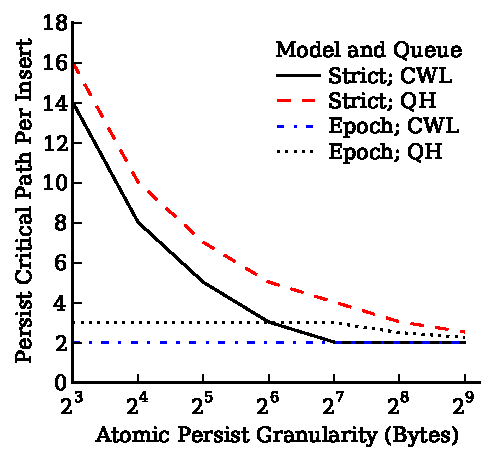
\includegraphics[width=.55\linewidth]{PersistencyEval/Coalescing.pdf}
  \caption{\textbf{Atomic Persist Size.} 1 Thread. Large atomic persists allow coalescing, increasing persist concurrency.  While effective for strict persistency, large atomic persists do not improve persist concurrency for relaxed models.}
  \label{fig::Coalescing}
\end{figure}


Figure~\ref{fig::Coalescing} displays average persist ordering critical path per insert for \emph{Copy While Locked} and \emph{Queue Holes} for both strict persistency and epoch persistency as atomic persist size increases from eight to 512 bytes.
At eight-byte persists there is a large separation between strict persistency and epoch persistency.
As atomic persist size increases the persist critical path of strict persistency steadily decreases while the critical path of epoch persistency remains largely unchanged.
At 512-byte atomic persists (right of the Figure) strict persistency matches epoch persistency.
For these queue benchmarks larger atomic persists provide the same improvement to persist critical path as relaxed persistency, but offer no improvement to relaxed models.
Increasing atomic persist granularity offers an alternative to relaxed persistency models.

\textbf{Persist False Sharing.}
Just as in existing memory systems, persists suffer from false sharing, degrading performance.
False sharing traditionally occurs under contention to the same cache line even though threads access disjoint addresses in that cache line.
Similarly, \emph{persistent false sharing} occurs when a persist ordering constraint is unnecessarily introduced due to the coarseness at which races are observed.
Persistent false sharing occurs in races to both persistent and volatile memory, as races to both address spaces establish persist ordering constraints.

 \begin{figure}
  \centering
  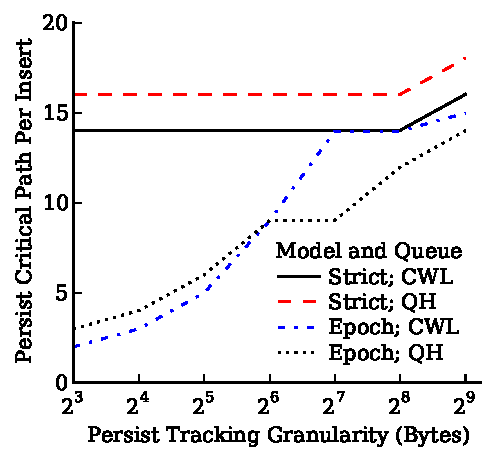
\includegraphics[width=.55\linewidth]{PersistencyEval/FalseSharing.pdf}
  \caption{\textbf{Persistent False Sharing.} 1 Thread.  False sharing negligably affects strict persistency (persists already serialized); relaxed models reintroduce constraints.}
  \label{fig::FalseSharing}
\end{figure}


Figure~\ref{fig::FalseSharing} shows average persist critical path per insert for \emph{Copy While Locked} and \emph{Queue Holes} for both strict persistency and epoch persistency as the granularity at which persist ordering constraints propagate increases.
For fine-grained tracking epoch persistency provides a far lower persist critical path than strict persistency.
As tracking granularity increases, strict persistency performance remains the same while epoch persistency decreases (critical path increases).
At 512-byte tracking granularity strict persistency and epoch persistency provide comparable persist critical paths; many of the persist constraints removed by relaxing consistency are reintroduced through false sharing.

\section{Future Work}
\label{sec:PersistencyEval:FutureWork}

This dissertation lays the foundation for reasoning about NVRAM performance and programming interfaces, culminating in memory persistency.
However, I leave it to future work to investigate how best to use persistency to build recoverable systems with NVRAM.

\textbf{Software for NVRAM.}
NVRAM should eventually allow data structures with the performance of existing DRAM systems but that recover after failures.
Such software will require transformations to introduce logs or indirection, and to properly order writes.
These transformations slow execution on even volatile memory systems.
However, an instruction-direct memory interface holds the potential to improve execution beyond block and transaction interfaces by increasing thread concurrency and removing frequent copies inherent in block storage interfaces.

New data structures must be developed to bridge the gap between existing high performance main-memory versions and those that provide recovery with disk.
For example, ordered indexes are typically implemented as B+Trees with disk, but novel (and complicated) variations exist for main memory, such as highly concurrent balanced trees and lock-free skip lists.
With NVRAM and memory persistency one might imagine a recoverable lock-free tree or skip list with bounded recovery time.
How to design such data structures remains uncertain, as does their true performance potential.

\textbf{New models and hardware implementations.}
Once software has been designed we will require hardware implementations of persistency models and NVRAM memory systems.
Existing memory consistency encompasses a broad literature of models and implementations, detailing specific relaxations to improve performance.
High performance techniques involving speculation further improve performance for strict consistency models.
The same will be true for persistency models, yet I expect persistency models must be further relaxed compared to consistency models (an NVRAM persist may take an order of magnitude longer than making a store visible to other processors).
Akin to speculation, logging and indirection (such as copy-on-write) may improve performance of strict persistency models.

Designing high performance and highly concurrent data structures, even without regard for persistency, remains a challenge.
To simplify matters researchers have introduced ``programmer-centric" memory consistency models---models that provide the appearance of SC when certain criteria are met (e.g., data-race-free-zero \cite{Adve96}).
Memory persistency may be similarly simplified by identifying programming patterns and the minimal synchronization constructs to present the appearance of SC while still giving the compiler and processor as much freedom as possible to reorder persists.

\textbf{Implementing efficient persist coalescing.}
Finally, the previous chapters assume that coalescing will be an important feature of NVRAM systems; indeed, recent work has already demonstrated that without hardware coalescing the software must cache and coalesce persists, introducing additional instructions and increasing the likelihood of design errors \cite{ConditNightingale09,FangHsiao11}.
Coalescing presents several problems such as detecting when coalescing is allowable and determining how long persists should be delayed (delaying a persist increases the chance that it will coalesce with future persists, but may delay important events such as transaction commit).
Future work must investigate language, compiler, and hardware mechanisms to provide persist coalescing.
It is possible for coalescing to occur only under specific conditions (e.g., coalescing only occurs between persists on the same thread, coalescing only occurs to a limited number of addresses labeled by the programmer), reducing hardware complexity.

\section{Conclusion}
\label{sec:PersistencyEval:Conclusion}

Future NVRAM technologies offer the performance of DRAM with the durability of disk.
However, existing memory interfaces are incapable of guaranteeing proper data recovery by properly enforcing persist order.
In previous chapters I introduced \emph{memory persistency}, an extension to memory consistency that allows programmers to describe persist order constraints.
Additionally, I outlined the design space of possible memory persistency models and detailed three persistency models and their use in implementing a persistent queue.
In this chapter I use memory tracing and simulation to demonstrate that strict persistency models suffer a 30$\times$ slowdown relative to instruction execution rate, and that relaxed persistency effectively regains this performance.
Memory persistency represents a framework for defining programmer interfaces for NVRAM and reasoning about program correctness for recoverable applications.
